\documentclass[11pt,letterpaper]{article}

%%%%%%%%%%%%%%%%%%%%%%%%%%%%%%%%%%%
% IMPORTACIÓN DE CONFIGURACIONES
%%%%%%%%%%%%%%%%%%%%%%%%%%%%%%%%%%%

%%%%%%%%%%%%%%%%%%%%%%%%%%%%
% PAQUETES
%%%%%%%%%%%%%%%%%%%%%%%%%%%%

\usepackage[utf8]{inputenc}                % Codificación UTF-8 para caracteres especiales
\usepackage[T1]{fontenc}                   % Mejora la salida de texto con acentos
% Babel no está disponible en esta instalación de TeX; se desactiva para que el documento compile.
% Si deseas activar el idioma español, instala el paquete correspondiente del sistema TeX y descomenta la línea:
% \usepackage[spanish]{babel}
\usepackage{graphicx}                      % Manejo avanzado de imágenes [\includegraphics]
\usepackage{float}                         % Posicionamiento preciso de figuras/tablas [H]
\usepackage{bookmark}                      % Bookmarks interactivos en PDF (mejorado)
\usepackage[makeroom]{cancel}              % Cancelación de términos en ecuaciones [\cancel]
\usepackage{hyperref}                      % Hipervínculos interactivos
\usepackage{nameref}                       % Referencias por nombre de sección
\usepackage{theoremref}                    % Referencias a teoremas mejoradas
\hypersetup{
    pdftitle={Assignment},                 % Metadatos del PDF
    colorlinks=true,                       % Enlaces en color (no recuadros)
    linkcolor=cyan!90,                     % Color enlaces internos
    urlcolor=blue,                         % Color URLs externas
    bookmarksnumbered=true,                % Numeración automática de bookmarks
    bookmarksopen=true                     % Bookmarks expandidos por defecto
}

\usepackage{amsmath, amsfonts, amsthm, amssymb, mathtools} % Base para matemáticas
\usepackage{xfrac}                         % Fracciones diagonales [\sfrac]
\usepackage{tikz-cd}                       % Diagramas conmutativos
\usepackage{tikzsymbols}                   % Símbolos especiales (emojis, misc.)
\usepackage{siunitx}                       % Alineación numérica en tablas [S]
\usepackage{multicol}                      % Columnas múltiples en texto/matemáticas

\usepackage{booktabs}                      % Reglas profesionales para tablas [\toprule]
\usepackage{array}                         % Control avanzado de columnas en tablas
\usepackage[ruled,vlined,linesnumbered]{algorithm2e} % Escritura de algoritmos
\usepackage[most,many,breakable]{tcolorbox} % Cajas decoradas con estilo
\usepackage{xcolor}                         % Gestión avanzada de colores
\usepackage{varwidth}                       % Cajas de ancho variable
\usepackage{enumitem}                       % Personalización de listas [nosep]
\usepackage{etoolbox}                      % Utilidades para programación LaTeX
\usepackage{import}                        % Importación modular de archivos
\usepackage{xifthen}                       % Condicionales en documentos
\usepackage{pdfpages}                     % Inclusión de páginas PDF externas
\usepackage{transparent}                  % Manejo de transparencias
% `babelbib` requiere soporte de idioma de babel, que no está instalado en este sistema.
% Se desactiva para que el documento compile sin errores.
% \usepackage[fixlanguage]{babelbib}
% \bibliographystyle{babunsrt}
\usepackage{titlesec}
% Personalización de títulos
% Centrar secciones automáticamente
\titleformat{\section}
  {\normalfont\Large\bfseries\centering}{\thesection}{1em}{}
\titleformat{\subsection}
  {\normalfont\large\bfseries\centering}{\thesubsection}{1em}{}

\usepackage{comment}  
\usepackage{epsfig, graphicx} % Inclusión de imágenes y gráficos
\usepackage[left=2cm, right=2cm, top=1.8cm, bottom=2.3cm]{geometry} % Define los márgenes del documento
\usepackage{fancyhdr}         % Para personalizar encabezados y pies de página
\usepackage{lastpage}         % Permite referenciar el número total de páginas
\usepackage{lipsum}           % Genera texto aleatorio para pruebas
\usepackage{pgfplots, mathtools}


%%%%%%%%%%%%%%%%%%%%%%%%%%%%
% COLORES
%%%%%%%%%%%%%%%%%%%%%%%%%%%%

\definecolor{mygr}{HTML}{2C3338}
\definecolor{mauve}{rgb}{0.58,0,0.82}  % Color morado

%%%%%%%%%%%%%%%%%%%%%%%%%%%%
% CAJAS
%%%%%%%%%%%%%%%%%%%%%%%%%%%%

% --------------------------
% Caja de Introducción/Indicaciones
% --------------------------
\newtcolorbox{intro}[1][]{%
    enhanced,                               % Habilitar mejoras gráficas
    before skip=2mm, after skip=2mm,        % Espaciado vertical
    colback=gray!5,                         % Color de fondo claro
    colframe=black!80!black,                % Borde oscuro
    boxrule=0.5mm,                          % Grosor del borde
    attach boxed title to top left={         % Posición del título
        xshift=1cm,                         % Desplazamiento horizontal
        yshift*=1mm-\tcboxedtitleheight      % Ajuste vertical preciso
    },
    varwidth boxed title*=-3cm,             % Ancho adaptable del título
    boxed title style={                     % Estilo personalizado del título
        frame code={                        % Diseño del marco del título
            \path[fill=tcbcolback]
            ([yshift=-1mm,xshift=-1mm]frame.north west)
            arc[start angle=0,end angle=180,radius=1mm]
            ([yshift=-1mm,xshift=1mm]frame.north east)
            arc[start angle=180,end angle=0,radius=1mm];
            \path[left color=tcbcolback!60!black,
                  right color=tcbcolback!60!black,
                  middle color=tcbcolback!80!black]
            ([xshift=-2mm]frame.north west) -- ([xshift=2mm]frame.north east)
            [rounded corners=1mm]-- ([xshift=1mm,yshift=-1mm]frame.north east)
            -- (frame.south east) -- (frame.south west)
            -- ([xshift=-1mm,yshift=-1mm]frame.north west)
            [sharp corners]-- cycle;
        }, 
        interior engine=empty,              % Sin relleno adicional
    },
    fonttitle=\bfseries,                    % Título en negrita
    title={Indicaciones},                   % Texto predeterminado del título
    #1                                      % Permite personalización adicional
}

% --------------------------
% Caja de Bibliografía (similar a intro con título diferente)
% --------------------------
\newtcolorbox{biblio}[1][]{enhanced,
    before skip=2mm, after skip=2mm, colback=gray!5, colframe=black!80!black, boxrule=0.5mm,
    attach boxed title to top left={xshift=1cm, yshift*=1mm-\tcboxedtitleheight}, varwidth boxed title*=-3cm,
    boxed title style={frame code={
            \path[fill=tcbcolback]
            ([yshift=-1mm,xshift=-1mm]frame.north west)
            arc[start angle=0,end angle=180,radius=1mm]
            ([yshift=-1mm,xshift=1mm]frame.north east)
            arc[start angle=180,end angle=0,radius=1mm];
            \path[left color=tcbcolback!60!black,right color=tcbcolback!60!black,
                middle color=tcbcolback!80!black]
            ([xshift=-2mm]frame.north west) -- ([xshift=2mm]frame.north east)
            [rounded corners=1mm]-- ([xshift=1mm,yshift=-1mm]frame.north east)
            -- (frame.south east) -- (frame.south west)
            -- ([xshift=-1mm,yshift=-1mm]frame.north west)
            [sharp corners]-- cycle;
        }, interior engine=empty,
    },
    fonttitle=\bfseries,
    title={Bibliografía}, #1
}

% --------------------------
% Caja de Inciso
% --------------------------
\makeatletter
\newtcolorbox{inciso}[2][]{%
    enhanced,
    breakable,
    colback=white,
    colframe=mygr,
    attach boxed title to top left={
        yshift*=-\tcboxedtitleheight
    },
    fonttitle=\bfseries,
    title={#2},
    boxed title size=title,
    boxed title style={
        sharp corners,
        rounded corners=northwest,
        colback=tcbcolframe,
        boxrule=0pt,
    },
    underlay boxed title={
        \path[fill=tcbcolframe] (title.south west)--(title.south east)
        to[out=0, in=180] ([xshift=5mm]title.east)--
        (title.center-|frame.east)
        [rounded corners=\kvtcb@arc] |-
        (frame.north) -| cycle;
    },
    #1
}
\makeatother

% --------------------------
% Caja de Notas
% --------------------------
\usetikzlibrary{arrows,calc,shadows.blur}   % Requisitos para efectos gráficos
\tcbuselibrary{skins}                       % Habilita skins avanzados

\newtcolorbox{notas}[1][]{%
    enhanced jigsaw,                        % Skin mejorado para efectos
    colback=gray!20!white,                  % Fondo gris claro
    colframe=gray!80!black,                 % Borde gris oscuro
    size=small,                             % Tamaño compacto
    boxrule=1pt,                            % Grosor del borde
    title=\textbf{Notas | Observaciones},   % Título doble
    halign title=flush center,              % Alineación central del título
    coltitle=black,                         % Color del texto del título
    breakable,                              % Permite dividir en páginas
    drop shadow=black!50!white,             % Sombra exterior
    attach boxed title to top left={         % Posición del título
        xshift=1cm,
        yshift=-\tcboxedtitleheight/2,
        yshifttext=-\tcboxedtitleheight/2
    },
    minipage boxed title=5cm,               % Ancho máximo del título
    boxed title style={                     % Estilo personalizado del título
        colback=white,                      % Fondo blanco
        size=fbox,                         % Tamaño tipo marco
        boxrule=1pt,                        % Grosor del borde
        boxsep=2pt,                         % Espaciado interno
        underlay={                          % Elementos gráficos bajo el título
            \coordinate (dotA) at ($(interior.west) + (-0.5pt,0)$);
            \coordinate (dotB) at ($(interior.east) + (0.5pt,0)$);
            \begin{scope}
                \clip (interior.north west) rectangle ([xshift=3ex]interior.east);
                \filldraw [white, blur shadow={shadow opacity=60, shadow yshift=-.75ex}, 
                          rounded corners=2pt] (interior.north west) rectangle (interior.south east);
            \end{scope}
            \begin{scope}[gray!80!black]
                \fill (dotA) circle (2pt);  % Punto decorativo izquierdo
                \fill (dotB) circle (2pt);  % Punto decorativo derecho
            \end{scope}
        },
    },
    #1                                      % Personalización adicional
}

% --------------------------
% Caja de Demostración
% --------------------------
\newtcbtheorem[]{demostracion}{Demostracion}%
{ enhanced,
  colback       = black!5,               % Color de fondo del recuadro
  colbacktitle  = black!5,               % Color de fondo del título
  coltitle      = black,                  % Color del texto del título
  boxrule       = 0pt,                    % Ancho del borde del recuadro
  frame hidden,                           % Oculta el marco del recuadro
  borderline west = {0.5mm}{0.0mm}{black},% Línea decorativa en el lateral izquierdo
  fonttitle     = \bfseries\sffamily,      % Fuente y estilo del título
  breakable,                              % Permite que el recuadro se divida en varias páginas
  before skip   = 3ex,                    % Espacio antes del entorno
  after skip    = 3ex                     % Espacio después del entorno
}{problem}


%%%%%%%%%%%%%%%%%%%%%%%%%%%%
% CONFIGURACIONES
%%%%%%%%%%%%%%%%%%%%%%%%%%%%

% Fallback para que el documento compile aunque babel no esté instalado.
\providecommand{\spanishdecimal}[1]{ }
% Ajusta el espaciado antes y después de los títulos de capítulos y secciones.
\titlespacing*{\chapter}{0cm}{-2.0cm}{0.50cm} % {izquierda}{espacio antes}{espacio después}
\titlespacing*{\section}{0cm}{0.50cm}{0.25cm}

% Configura la indentación y separación entre párrafos.
\setlength{\parindent}{0pt}  % Sin indentación en los párrafos
\setlength{\parskip}{1ex}    % Espacio extra entre párrafos


% Configuración de encabezados y pies con fancyhdr.
\pagestyle{fancy}
\fancyhf{}  % Limpia los encabezados y pies predeterminados
\rfoot{%
  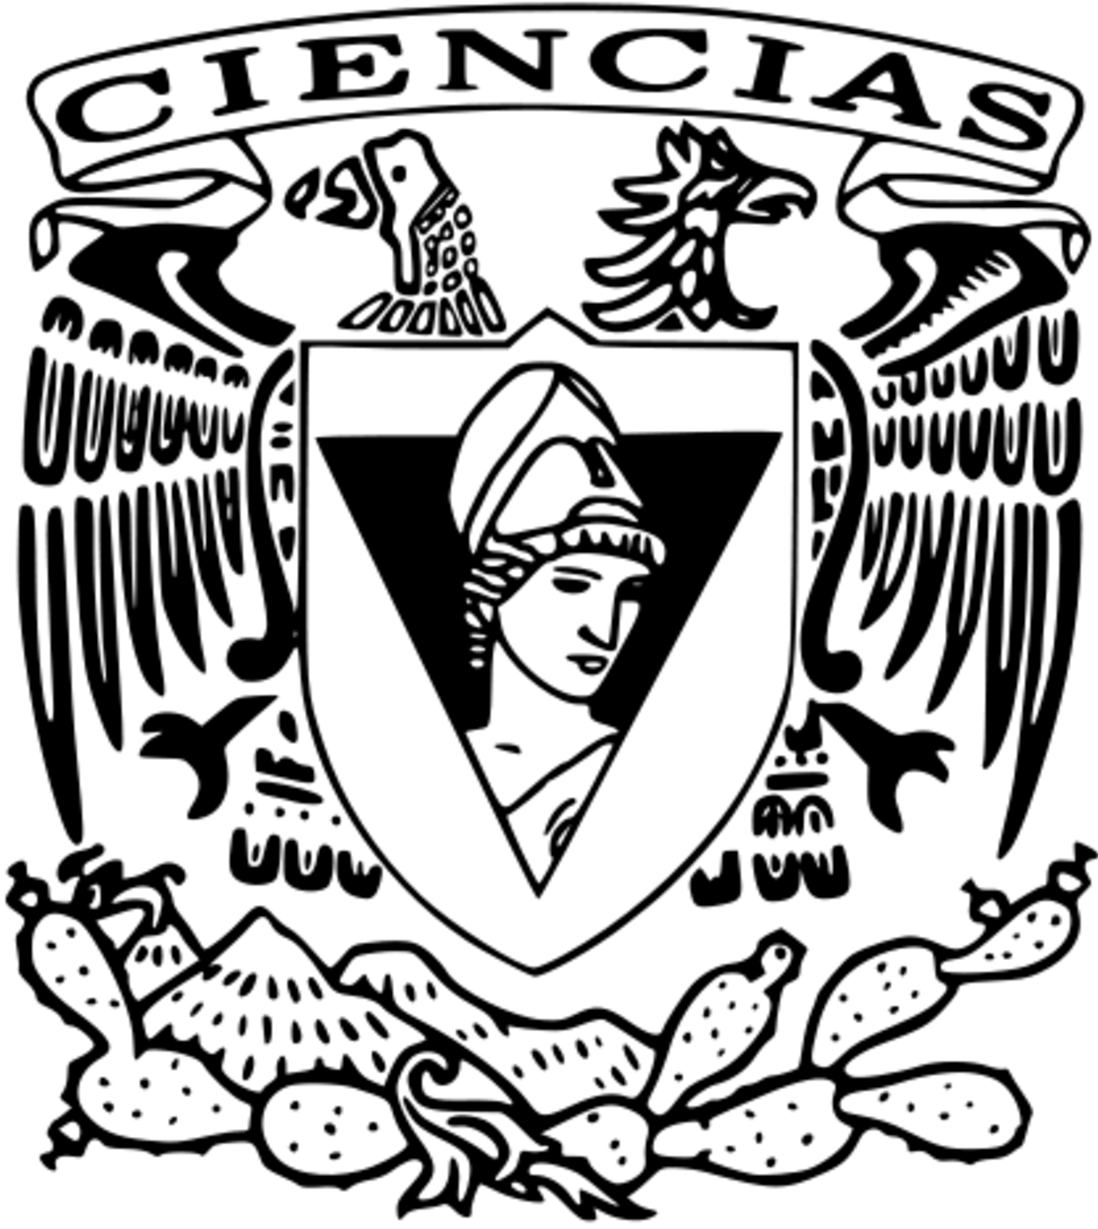
\includegraphics[height=1cm]{Logo_FC.png} \hfill % Inserta un logo a la derecha
  \textit{Página \thepage\ de \pageref{LastPage}}
}

\usetikzlibrary{arrows, backgrounds, shapes.arrows, positioning} % Librerías de TikZ para gráficos vectoriales
\pgfplotsset{compat=newest}   % Asegura la compatibilidad con la versión más reciente de pgfplots

%%%%%%%%%%%%%%%%%%%%%%%%%%%%
% DEFINICIÓN DE ENTORNOS Y COMANDOS
%%%%%%%%%%%%%%%%%%%%%%%%%%%%

% definición del operador para \left( \right)
\newcommand{\paren}[1]{\left({#1}\right)}

% definición del operador para derivada
\newcommand{\dd}[2]{\dfrac{\mathrm{d}#1}{\mathrm{d}#2}}

% definición del operador para la función techo
\newcommand{\techo}[1]{\lceil {#1} \rceil}

% Redefine la numeración de listas para usar números (permite contadores más grandes que el sistema alfabético).
\renewcommand{\theenumi}{\arabic{enumi})}

% Comandos personalizados para mejorar la notación matemática.
\let\emptyset\varnothing         % Utiliza el símbolo \varnothing para el conjunto vacío
\newcommand{\lto}{\mathbin{\to}}   % Define un comando para la flecha "→"

% Redefine los operadores de parte real e imaginaria para evitar conflictos.
\let\Re\relax
\DeclareMathOperator{\Re}{Re}
\let\Im\relax
\DeclareMathOperator{\Im}{Im}

% Definición de entornos para teoremas, corolarios, definiciones y proposiciones.
\newtheorem{teorema}{Teorema}
\newtheorem{corolario}{Corolario}
\newtheorem{definición}{Definición}
\newtheorem{proposición}{Proposición}

%%%%%%%%%%%%%%%%%%%%%%%%%%%%
% INICIO DE DOCUMENTO
%%%%%%%%%%%%%%%%%%%%%%%%%%%%

\begin{document}

%%%%%%%%%%%%%%%%%%%%%%%%%%%%
% ENCABEZADO
%%%%%%%%%%%%%%%%%%%%%%%%%%%%
\begin{center}
    \begin{minipage}{3cm}
    	\begin{center}
    		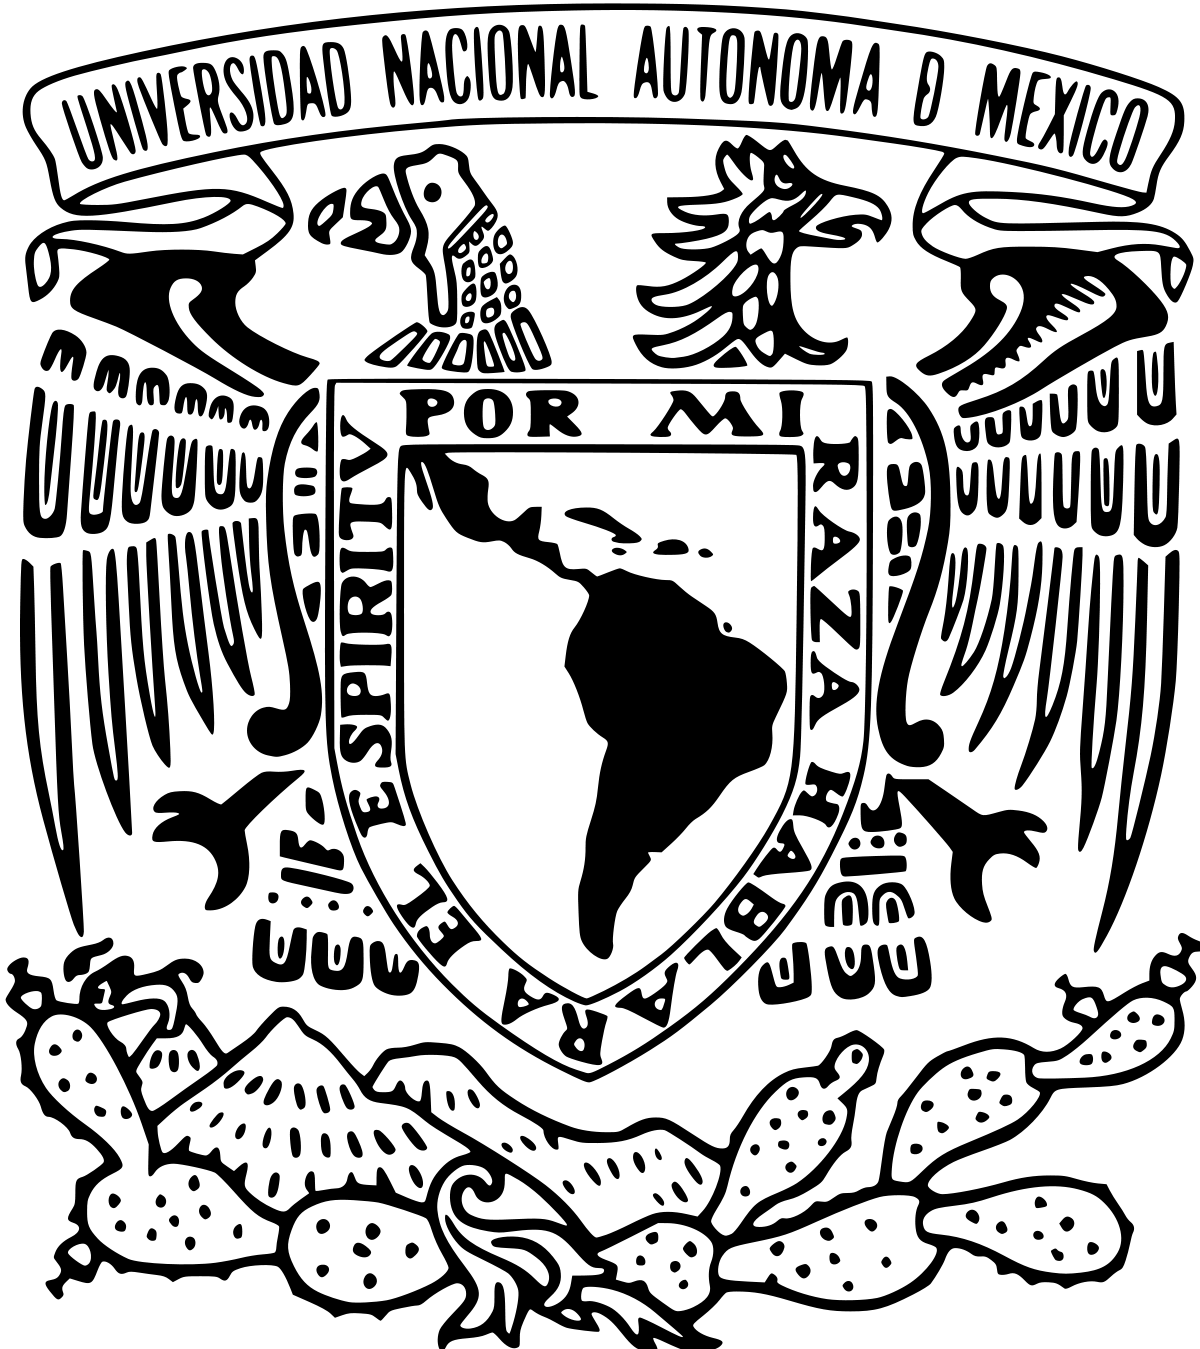
\includegraphics[height=3.4cm]{Logo_UNAM.png}
    	\end{center}
    \end{minipage}\hfill
    \begin{minipage}{10cm}
    	\begin{center}
    	\textbf{\large Universidad Nacional Autónoma de México}\\[0.1cm]
        \textbf{Facultad de Ciencias}\\[0.1cm]
        \textbf{Fenómenos Colectivos}\\[0.1cm]
        Tarea 1\\[0.1cm]
        Martínez Castro Alvaro Leonardo\\[0.1cm]
        \today
    	\end{center}
    \end{minipage}\hfill
    \begin{minipage}{3cm}
    	\begin{center}
    		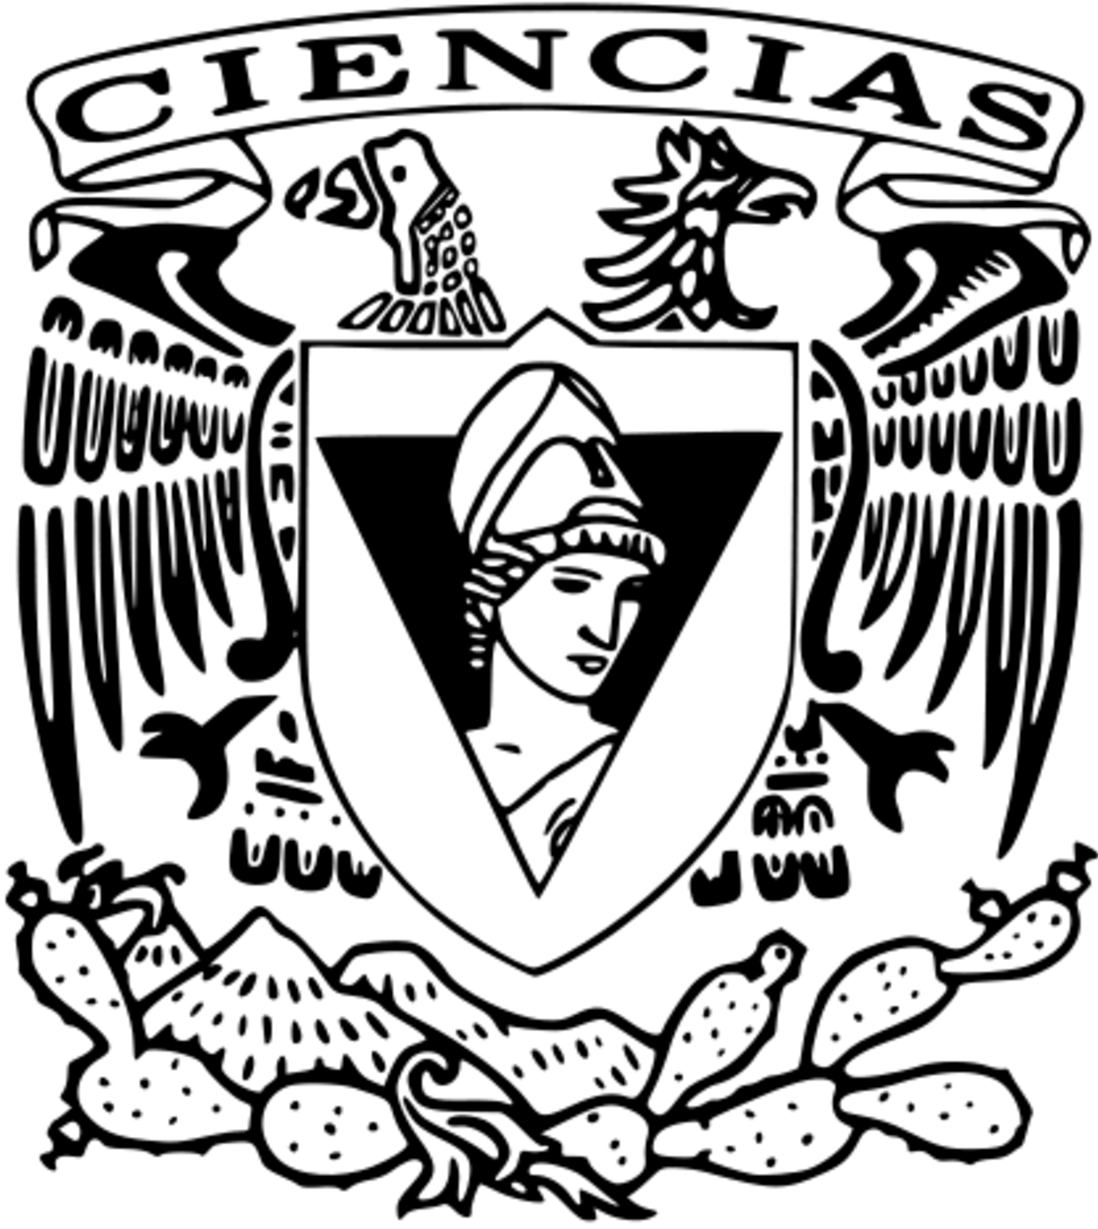
\includegraphics[height=3.4cm]{Logo_FC.png}
    	\end{center}
    \end{minipage}
\end{center}

\rule{17cm}{0.1mm}

%%%%%%%%%%%%%%%%%%%%%%%%%%%%
% FIN DE ENCABEZADO
%%%%%%%%%%%%%%%%%%%%%%%%%%%%

\begin{inciso}{Inciso 1}
La temperatura es fundamentalmente un concepto macroscópico. En el marco de la termodinámica clásica, se define a través de la Ley Cero como la propiedad de estado común que determina si dos o más sistemas se encuentran en equilibrio térmico entre sí.

Aunque la física estadística permite conectar esta cantidad con el promedio de la energía cinética traslacional de las partículas, la temperatura carece de sentido si se intenta aplicar a una sola molécula o a un sistema con muy pocos grados de libertad. Para que el concepto esté físicamente bien definido y las fluctuaciones de energía sean despreciables respecto al valor medio, se requiere el límite termodinámico, es decir, que el número de partículas sea muy grande ($N \to \infty$).
\end{inciso}
\begin{inciso}{Inciso 2}
Para medir la temperatura de un sistema es necesario ponerlo en contacto térmico con el termómetro y esperar a que alcancen el equilibrio. Durante este proceso ocurre una transferencia neta de calor $Q$ entre ambos cuerpos. Con el fin de que la medición no altere significativamente el estado original de la muestra, la capacidad calorífica del instrumento ($C_{\text{term}}$) debe ser despreciable en comparación con la del sistema a medir ($C_{\text{sistema}}$).

En este caso, un dedal contiene una masa $m$ de agua sumamente pequeña, por lo que su capacidad térmica total, dada por $C = mc$, es muy reducida. Por el contrario, un termómetro de vidrio de tamaño estándar posee una masa considerable y una capacidad calorífica comparable o incluso mayor que la del agua en el dedal. Al ponerlos en contacto, el termómetro absorberá una cantidad importante de calor, enfriando de forma drástica el líquido. Como resultado, la temperatura final de equilibrio ($T_{\text{eq}}$) que marque el instrumento será muy diferente de la temperatura inicial que realmente se quería registrar.
\end{inciso}
\begin{inciso}{Inciso 3}
En principio y desde un punto de vista teórico, cualquier gas sirve como sustancia termométrica si se opera en el límite de bajas presiones ($P \to 0$). En este régimen, todos los gases reales tienden asintóticamente al comportamiento del gas ideal descrito por $PV = nRT$, lo que permite que la escala de temperatura resulte independiente del fluido empleado.

Sin embargo, a nivel experimental sí existen gases mejores que otros. Las propiedades deseables en el gas son, en primer lugar, tener temperaturas de licuefacción y solidificación extremadamente bajas, garantizando así que la sustancia permanezca en fase gaseosa durante mediciones criogénicas. En segundo lugar, conviene que tenga una baja densidad y fuerzas intermoleculares mínimas, lo que reduce las desviaciones del comportamiento ideal a presiones finitas.

Por estas razones, el helio ($\text{He}$) y el hidrógeno molecular ($\text{H}_{2}$) son los fluidos óptimos para el termómetro de gas a volumen constante. El helio resulta especialmente superior debido a que no condensa sino hasta cerca de $4\text{ K}$ a presión estándar, proporcionando el intervalo útil de medición más amplio.
\end{inciso}
\begin{inciso}{Inciso 4}
Dado que la variación de la fuerza electromotriz $\varepsilon$ con respecto a la temperatura $T$ es lineal, podemos modelar el comportamiento del termopar mediante la función $\varepsilon(T) = \alpha T + \beta$, donde $\alpha$ y $\beta$ son constantes por determinar a partir de las condiciones dadas. 

A partir de los datos, sabemos que a $0^\circ\text{C}$ la salida es de $0\text{ mV}$, por lo que directamente se deduce que $\beta = 0$. Además, a $510^\circ\text{C}$ el voltaje alcanza los $28\text{ mV}$, lo que nos permite obtener el valor de la pendiente:
\begin{equation*}
    \alpha = \frac{28\text{ mV}}{510^\circ\text{C}} = \frac{14}{255}\,\frac{\text{mV}}{^\circ\text{C}}
\end{equation*}
Con esto, la relación de calibración queda expresada como $\varepsilon(T) = \left(\frac{14}{255}\right) T$.

Para determinar la temperatura de la unión cuando el termopar registra una lectura de $10.2\text{ mV}$, sustituimos el voltaje y despejamos $T$:
\begin{align*}
    10.2 &= \left(\frac{14}{255}\right) T \\
    T &= \frac{10.2 \times 255}{14} \approx 185.79^\circ\text{C}
\end{align*}
Por lo tanto, la temperatura en la unión variable corresponde a $185.79^\circ\text{C}$.
\end{inciso}
\begin{inciso}{Inciso 5}
Para encontrar las temperaturas en las que dos escalas coinciden numéricamente, basta con plantear la condición de igualdad $T_1 = T_2 = x$ en las ecuaciones de conversión respectivas y despejar la incógnita.

Para las escalas Fahrenheit y Celsius, partimos de la relación $T_F = \frac{9}{5}T_C + 32$. Al imponer que $T_F = T_C = x$, agrupamos los términos algebraicos:
\begin{align*}
    x &= \frac{9}{5}x + 32 \\
    x - \frac{9}{5}x &= 32 \\
    -\frac{4}{5}x &= 32 \\
    x &= \frac{32 \times (-5)}{4} = -40
\end{align*}
De este modo, ambas escalas dan exactamente la misma lectura a una temperatura de $-40^\circ\text{C}$ (o $-40^\circ\text{F}$).

Para las escalas Fahrenheit y Kelvin, utilizamos la relación de transformación $T_F = \frac{9}{5}(T_K - 273.15) + 32$. Igualando ambas lecturas a $x$:
\begin{align*}
    x &= \frac{9}{5}(x - 273.15) + 32 \\
    x &= 1.8x - 491.67 + 32 \\
    -0.8x &= -459.67 \\
    x &= \frac{-459.67}{-0.8} \approx 574.59
\end{align*}
Por consiguiente, la lectura numérica coincide a los $574.59\text{ K}$ (o $574.59^\circ\text{F}$).

Finalmente, para las escalas Celsius y Kelvin, la transformación viene dada por el desplazamiento del cero: $T_K = T_C + 273.15$. Si intentamos imponer la condición $x = x + 273.15$, llegamos a la contradicción $0 = 273.15$. Como ambas funciones corresponden a rectas paralelas con la misma pendiente, no existe ningún punto de intersección; es decir, no hay ninguna temperatura en la que las lecturas de Celsius y Kelvin coincidan.
\end{inciso}
\begin{inciso}{Inciso 6}
Partiendo nuevamente de la conversión general $T_F = \frac{9}{5}T_C + 32$, analizamos las relaciones de proporción solicitadas para encontrar la temperatura correspondiente.

En el caso donde la lectura en Fahrenheit sea el doble que en Celsius ($T_F = 2T_C$), sustituimos directamente la condición en la fórmula:
\begin{align*}
    2T_C &= \frac{9}{5}T_C + 32 \\
    2T_C - 1.8T_C &= 32 \\
    0.2T_C &= 32 \\
    T_C &= \frac{32}{0.2} = 160^\circ\text{C}
\end{align*}
La lectura en Fahrenheit es el doble de la de Celsius a $160^\circ\text{C}$, lo que equivale a una lectura de $320^\circ\text{F}$.

Por otro lado, cuando la lectura en Fahrenheit es la mitad de la lectura en Celsius ($T_F = \frac{1}{2}T_C$), planteamos:
\begin{align*}
    \frac{1}{2}T_C &= \frac{9}{5}T_C + 32 \\
    0.5T_C - 1.8T_C &= 32 \\
    -1.3T_C &= 32 \\
    T_C &= -\frac{32}{1.3} \approx -24.62^\circ\text{C}
\end{align*}
Así, la relación se cumple aproximadamente a los $-24.62^\circ\text{C}$, lo que corresponde a una lectura de $-12.31^\circ\text{F}$.
\end{inciso}
\begin{inciso}{Inciso 7}
\textbf{a)} Sabemos que la dilatación térmica lineal se describe con la relación $\Delta L = \alpha L_{0} \Delta T$. Según los datos del problema, el cambio fraccional de longitud es $\Delta L / L_{0} = 0.00092$ para un cambio de temperatura de $\Delta T = 40^{\circ}\text{C}$. Despejando $\alpha$ tenemos:
\begin{equation*}
    \alpha = \frac{\Delta L / L_{0}}{\Delta T} = \frac{0.00092}{40^{\circ}\text{C}} = 2.3 \times 10^{-5} \, ^{\circ}\text{C}^{-1}
\end{equation*}

Luego, para encontrar el cambio en la densidad $\rho = m/V$, usamos la dilatación volumétrica. Como suponemos un material isótropo, el coeficiente de dilatación volumétrica es $\beta \approx 3\alpha$. El volumen final se expresa como $V = V_{0}(1 + \beta \Delta T)$. Dado que la masa se conserva, la densidad final queda así:
\begin{equation*}
    \rho = \frac{m}{V_{0}(1 + \beta \Delta T)} = \rho_{0}(1 + \beta \Delta T)^{-1}
\end{equation*}

Si expandimos esto con una serie de Taylor y nos quedamos a primer orden (ya que $\beta \Delta T$ es muy pequeño), obtenemos la aproximación $\rho \approx \rho_{0}(1 - \beta \Delta T)$. Entonces, el cambio fraccional de la densidad es:
\begin{equation*}
    \frac{\Delta \rho}{\rho_{0}} \approx -\beta \Delta T = -3\alpha \Delta T
\end{equation*}

Sustituyendo el valor que ya conocíamos de $\alpha \Delta T = 0.00092$, el cambio resulta en $-3(0.00092) = -0.00276$. Es decir, la densidad disminuye un $0.276\%$.

\textbf{b)} Con el coeficiente que calculamos, $\alpha = 2.3 \times 10^{-5} \, ^{\circ}\text{C}^{-1}$, y revisando las tablas de propiedades en los libros de texto, vemos que este valor corresponde al aluminio.
\end{inciso}
\begin{inciso}{Inciso 8}
La expansión del volumen exterior sería exactamente la misma para ambos cuerpos. Una manera sencilla de visualizarlo es imaginar el cuerpo hueco como si estuviera completamente relleno del mismo material. Al aumentar la temperatura, la distancia media entre los átomos aumenta de forma uniforme en todas direcciones. 

Si la cavidad estuviera llena, ese volumen interno se expandiría siguiendo la misma regla de $\Delta V = \beta V_{0} \Delta T$. Como al calentarse de manera uniforme no se generan tensiones térmicas extrañas, el material que rodea el hueco simplemente es empujado hacia afuera en esa misma proporción. Por lo tanto, el hueco crece en la misma medida que lo haría un núcleo sólido, lo que hace que por fuera los dos cuerpos se dilaten exactamente igual.
\end{inciso}
\begin{inciso}{Inciso 9}
La razón por la que no nos quemamos al meter la mano en el aire del horno a $200^{\circ}\text{C}$ tiene que ver con la forma en la que se transfiere el calor. El aire tiene una densidad y una conductividad térmica muy bajas, además de una capacidad calorífica mucho menor comparada con la de un metal sólido. 

Por esto, la cantidad de energía térmica que le pasa a nuestra piel por unidad de tiempo es muy pequeña. Al meter la mano, la capa de aire caliente que hace contacto directo con la piel le cede rápidamente su poca energía y se enfría, actuando casi como una capa aislante momentánea. En cambio, si tocáramos las paredes metálicas del horno, como son excelentes conductoras y mucho más densas, nos transferirían un flujo de calor constante y masivo que nuestra piel no podría disipar, provocando una quemadura inmediata.
\end{inciso}
\begin{inciso}{Inciso 10}
Durante un cambio de fase en una sustancia pura, el proceso ocurre de manera isotérmica, es decir, con $\Delta T = 0$. En este régimen, la energía transferida en forma de calor no se utiliza para aumentar la energía cinética promedio de las partículas (lo cual incrementaría la temperatura), sino que se invierte a nivel microscópico en vencer las fuerzas intermoleculares para reorganizar la estructura de la materia, modificando únicamente la energía potencial del sistema.

Si intentáramos emplear la definición habitual de calor específico:
\[
c = \frac{Q}{m \Delta T}
\]
al sustituir $\Delta T = 0$ obtendríamos una división por cero, lo que carece de sentido físico y matemático. Por esta razón, los calores latentes de fusión ($L_f$) y de vaporización ($L_v$) se definen de manera directa como la energía necesaria por unidad de masa para que ocurra el cambio de fase:
\[
Q = m L \implies L = \frac{Q}{m}
\]
A partir de este despeje es evidente que en el Sistema Internacional las unidades correspondientes son simplemente $\text{J/kg}$. No tiene sentido incluir un factor de $\text{K}^{-1}$, ya que durante la transición no interviene ninguna variación de temperatura.
\end{inciso}
\begin{inciso}{Inciso 11}
\textbf{a)} La capacidad calorífica $C$ se define termodinámicamente como el cociente entre el calor infinitesimal transferido al sistema y la variación de temperatura que este produce:
\[
C = \frac{\delta Q}{dT}
\]
Se trata de una propiedad extensiva que cuantifica cuánta energía térmica requiere todo el cuerpo para elevar su temperatura en una unidad, y sus unidades en el Sistema Internacional son $\text{J/K}$.

\vspace{0.8em}
\textbf{b)} No es correcto decir que un cuerpo ''contiene calor''. En termodinámica, los sistemas almacenan energía interna $U$, la cual sí es una función de estado que depende de variables como la temperatura y el volumen. El calor $Q$, de manera análoga al trabajo $W$, es energía en tránsito que cruza la frontera del sistema únicamente como resultado de una diferencia de temperatura con su entorno. Una vez transferida, pasa a sumarse o restarse de la energía interna, por lo que nunca hablamos de calor contenido, sino de calor intercambiado.

\vspace{0.8em}
\textbf{c)} La diferencia entre la dispersión de los calores específicos $c$ y la uniformidad de las capacidades caloríficas molares $C$ se explica mediante la ley de Dulong-Petit y el teorema de equipartición de la energía.

El calor específico $c$ mide la energía requerida por unidad de masa ($\text{kg}$). Dado que la masa molar $M$ difiere sustancialmente entre elementos (por ejemplo, el berilio tiene una masa atómica mucho menor que el plomo), un kilogramo de berilio contiene muchísimos más átomos que un kilogramo de plomo. Como consecuencia, calentar un kilogramo de un metal ligero requiere transferir calor a un número mucho mayor de partículas, lo que hace que los valores de $c$ varíen notablemente entre sustancias.

En contraste, la capacidad calorífica molar se define como $C = cM$, lo que equivale a normalizar la cantidad de materia a exactamente un mol ($N_A$ átomos), independientemente del elemento. En un sólido cristalino, cada átomo puede aproximarse como un oscilador armónico clásico en tres dimensiones, poseyendo 6 grados de libertad cuadráticos: 3 de energía cinética y 3 de energía potencial elástica.

Por el teorema de equipartición, a temperaturas ordinarias cada término cuadrático contribuye en promedio con $\frac{1}{2} k_B T$ a la energía del sistema. Multiplicando por los 6 grados de libertad y por el número de Avogadro $N_A$, la energía interna molar promedio del sólido resulta:
\[
U_m = 6 \left( \frac{1}{2} N_A k_B T \right) = 3 R T
\]
donde $R = N_A k_B$ es la constante universal de los gases. Derivando respecto a la temperatura, se obtiene la capacidad calorífica molar teórica:
\[
C = \frac{dU_m}{dT} = 3R \approx 3 \left(8.314 \, \frac{\text{J}}{\text{mol}\cdot\text{K}}\right) \approx 24.9 \, \frac{\text{J}}{\text{mol}\cdot\text{K}}
\]
Este resultado demuestra que la capacidad calorífica molar no depende de la masa inercial de los átomos, sino únicamente de la cantidad de osciladores en la red. Esto justifica que los valores experimentales de los distintos metales converjan a valores cercanos a $25 \, \text{J}/(\text{mol}\cdot\text{K})$.
\end{inciso}
\begin{inciso}{Inciso 12}
El cambio de fase de agua líquida a hielo no ocurre de golpe cuando la temperatura alcanza los $0\,^{\circ}\mathrm{C}$ porque no basta únicamente con llegar a la temperatura de congelación; para formar la estructura sólida, el agua necesita liberar una cantidad considerable de energía correspondiente al calor latente de fusión, regido por:
\[
Q = m L_f
\]
La extracción de esta energía no es instantánea, sino que depende de la tasa de transferencia de calor hacia el entorno (por conducción y convección). Como el flujo de calor toma un tiempo finito, el proceso no puede ser repentino.

Por este mismo motivo, el agua comienza a congelarse primero junto a las paredes de la bandeja. Estas zonas se encuentran en contacto térmico directo con el material del recipiente y el aire frío exterior, por lo que allí se establece el mayor gradiente de temperatura y el calor latente se disipa con mayor rapidez hacia afuera. El interior tarda más tiempo en congelarse debido a que el agua circundante y la capa inicial de hielo exterior funcionan como una barrera aislante.
\end{inciso}
\begin{inciso}{Inciso 13}
La razón por la que la Tierra no está en equilibrio térmico con el Sol se debe a la enorme distancia que los separa y al balance de radiación que se establece. Si existiera un equilibrio térmico estricto en el sentido de la Ley Cero, ambos cuerpos tendrían que compartir la misma temperatura, lo cual implicaría que la superficie terrestre se encontrara a los mismos $5800\,\mathrm{K}$ que la superficie solar.

Sin embargo, al estar separados por el vacío, el único mecanismo viable de transferencia de calor es la radiación electromagnética. La Tierra intercepta una fracción minúscula de la radiación emitida por el Sol debido al pequeño ángulo sólido que subtiende a esa distancia. A su vez, la Tierra no acumula energía de forma indefinida: irradia continuamente calor hacia el espacio exterior, el cual actúa como un sumidero térmico a aproximadamente $2.7\,\mathrm{K}$. Por ende, el planeta no está en equilibrio térmico con el Sol, sino en un estado estacionario donde la energía solar absorbida por unidad de tiempo se equilibra con la energía que el planeta emite al espacio, manteniendo una temperatura promedio estable.
\end{inciso}
\begin{inciso}{Inciso 14}
\textbf{a)} Para determinar la cantidad de calor necesaria para calentar el agua sin cambio de fase, utilizamos la expresión de calor sensible a presión constante:
\[
Q = m c \Delta T
\]
Tomando la masa de agua $m = 0.320\,\mathrm{kg}$, el calor específico del agua líquida $c = 4190\,\mathrm{J}/(\mathrm{kg}\cdot\mathrm{K})$ y la diferencia de temperatura $\Delta T = 80.0\,^{\circ}\mathrm{C} - 20.0\,^{\circ}\mathrm{C} = 60.0\,\mathrm{K}$, sustituimos los datos:
\[
Q = (0.320\,\mathrm{kg})\left(4190\,\frac{\mathrm{J}}{\mathrm{kg}\cdot\mathrm{K}}\right)(60.0\,\mathrm{K})
\]
\[
Q = 80448\,\mathrm{J} \approx 80.45\,\mathrm{kJ}
\]
Por lo tanto, se requiere suministrar $80448\,\mathrm{J}$ (o $80.45\,\mathrm{kJ}$) de calor al agua.

\textbf{b)} Suponiendo que toda la potencia de la resistencia de inmersión se invierte directamente en calentar el agua sin pérdidas hacia el vaso o los alrededores, la relación entre potencia, energía y tiempo es:
\[
P = \frac{Q}{\Delta t}
\]
Despejando el intervalo de tiempo $\Delta t$:
\[
\Delta t = \frac{Q}{P}
\]
Sustituyendo el calor obtenido en el inciso anterior y la potencia $P = 200\,\mathrm{W}$:
\[
\Delta t = \frac{80448\,\mathrm{J}}{200\,\mathrm{W}} = 402.24\,\mathrm{s}
\]
Si lo convertimos a minutos:
\[
\Delta t = \frac{402.24}{60}\,\mathrm{min} \approx 6.70\,\mathrm{min}
\]
Se requieren $402.24\,\mathrm{s}$ (aproximadamente $6.70\,\mathrm{min}$) para alcanzar los $80.0\,^{\circ}\mathrm{C}$.
\end{inciso}
\begin{inciso}{Inciso 15}
\textbf{a)} Sabemos que el periodo de un péndulo simple es $\tau = 2\pi\sqrt{L/g}$, donde $L$ es la longitud y $g$ la gravedad. Al pasar de $25^{\circ}\text{C}$ a $5^{\circ}\text{C}$, el cambio de temperatura es $\Delta T = -20\text{ K}$. Usando el coeficiente de dilatación lineal del acero ($\alpha = 1.2 \times 10^{-5}\text{ K}^{-1}$), el cambio fraccional en la longitud es $\Delta L / L_{0} = \alpha \Delta T$. Sustituyendo los datos:
$$ \frac{\Delta L}{L_{0}} = (1.2 \times 10^{-5}\text{ K}^{-1})(-20\text{ K}) = -2.4 \times 10^{-4} $$
El signo negativo nos indica que la barra se contrajo. 

\vspace{0.3cm}
\noindent\textbf{b)} Como cambió la longitud, el nuevo periodo $\tau'$ se puede aproximar usando una expansión de Taylor (ya que $\alpha \Delta T$ es muy pequeño comparado con 1):
$$ \tau' = 2\pi\sqrt{\frac{L_{0}(1 + \alpha \Delta T)}{g}} = \tau_{0} (1 + \alpha \Delta T)^{1/2} \approx \tau_{0} \left( 1 + \frac{1}{2}\alpha \Delta T \right) $$
Entonces, el cambio fraccional del periodo es $\Delta \tau / \tau_{0} \approx \frac{1}{2}\alpha \Delta T$. Considerando que un día tiene $t = 86400\text{ s}$, la diferencia de tiempo $\Delta t$ que registra el reloj es:
$$ \Delta t = -t \left( \frac{\Delta \tau}{\tau_{0}} \right) = -t \left( \frac{1}{2}\alpha \Delta T \right) $$
$$ \Delta t = -(86400\text{ s}) \left[ \frac{1}{2} (1.2 \times 10^{-5}\text{ K}^{-1}) (-20\text{ K}) \right] = +10.368\text{ s} $$
Como el péndulo se acortó, el reloj va más rápido y gana unos $10.4\text{ s}$ por día. 

\vspace{0.3cm}
\noindent\textbf{c)} Para que el reloj no gane ni pierda más de un segundo, necesitamos que $|\Delta t| \le 1\text{ s}$. Despejando la variación de temperatura $|\Delta T|$ de nuestra ecuación anterior:
$$ |\Delta t| = t \left( \frac{1}{2}\alpha |\Delta T| \right) \le 1\text{ s} \implies |\Delta T| \le \frac{2(1\text{ s})}{t \alpha} $$
$$ |\Delta T| \le \frac{2}{(86400\text{ s}) (1.2 \times 10^{-5}\text{ K}^{-1})} \approx 1.93\text{ K} $$
Por lo tanto, la temperatura ambiente del cuarto no debe variar más de $\pm 1.93^{\circ}\text{C}$ respecto a los $25^{\circ}\text{C}$ originales.
\end{inciso}
\begin{inciso}{Inciso 16}
Por conservación de la energía, suponemos que toda la energía cinética inicial de la bala se transforma en calor ($Q$) justo al detenerse. Este calor debe alcanzar para elevar la temperatura del plomo hasta su punto de fusión ($T_{f} = 327.3^{\circ}\text{C}$) y luego derretirlo por completo. Así que sumamos el calor sensible y el latente: $Q = mc\Delta T + mL_{f}$. Igualando esto con la energía cinética $K = \frac{1}{2}mv^{2}$, vemos que la masa $m$ se cancela:
$$ \frac{1}{2}mv^{2} = m(c\Delta T + L_{f}) \implies v = \sqrt{2(c\Delta T + L_{f})} $$
Para el plomo, sabemos que $c = 130\text{ J}/(\text{kg}\cdot\text{K})$ y $L_{f} \approx 24.5 \times 10^{3}\text{ J/kg}$. El cambio de temperatura es $\Delta T = 327.3^{\circ}\text{C} - 25.0^{\circ}\text{C} = 302.3\text{ K}$. Sustituyendo todo en la expresión de la velocidad:
$$ v = \sqrt{2 \left[ 130 (302.3) + 24.5 \times 10^{3} \right]} = \sqrt{2 (39299 + 24500)} = \sqrt{127598} $$
$$ v \approx 357.21\text{ m/s} $$
Como vemos, la rapidez necesaria es supersónica (mayor a los $347\text{ m/s}$ del sonido), lo cual tiene bastante sentido físico para generar tanto calor por fricción o impacto.
\end{inciso}
\begin{inciso}{Inciso 17}
Como el sistema está operando en estado estacionario, aplicamos la ley de conducción de Fourier unidimensional: $H = kA \frac{\Delta T}{L}$. El problema nos dice que el calor conducido en un tiempo de $\Delta t = 10.0\text{ min} = 600\text{ s}$ se usa por completo para derretir el hielo, así que lo relacionamos con el calor latente de fusión del agua ($L_{f} = 334 \times 10^{3}\text{ J/kg}$) usando $Q = mL_{f}$. La tasa de transferencia de calor $H = Q/\Delta t$ es:
$$ H = \frac{(8.50 \times 10^{-3}\text{ kg})(334 \times 10^{3}\text{ J/kg})}{600\text{ s}} = \frac{2839\text{ J}}{600\text{ s}} = 4.7317\text{ W} $$
Teniendo ya la corriente térmica $H$ y sabiendo que el área de la varilla es $A = 1.25\text{ cm}^{2} = 1.25 \times 10^{-4}\text{ m}^{2}$, podemos despejar la conductividad térmica $k$:
$$ k = \frac{H \cdot L}{A \cdot \Delta T} = \frac{(4.7317\text{ W})(0.600\text{ m})}{(1.25 \times 10^{-4}\text{ m}^{2})(100.0\text{ K})} = 227.12\text{ W}/(\text{m}\cdot\text{K}) $$
Este valor de $227.12\text{ W}/(\text{m}\cdot\text{K})$ corresponde empíricamente a la conductividad térmica de un metal como el aluminio.
\end{inciso}
\begin{inciso}{Inciso 18}
\noindent \textbf{a)} Para calcular la corriente de calor a través del aislante, consideramos que la transferencia ocurre en régimen estacionario unidimensional mediante la ley de conducción de Fourier:
\begin{equation*}
    H = k A \frac{\Delta T}{\Delta x}
\end{equation*}

\noindent De los datos del enunciado tenemos que el área de la pared es $A = 1.40\text{ m}^2$, el espesor de la capa de fibra de vidrio es $\Delta x = 4.00\text{ cm} = 0.0400\text{ m}$ y su conductividad térmica es $k = 0.040\text{ W}/(\text{m}\cdot\text{K})$. La diferencia de temperatura entre las superficies interior y exterior es:
\begin{equation*}
    \Delta T = 175^\circ\text{C} - 35.0^\circ\text{C} = 140^\circ\text{C} = 140\text{ K}
\end{equation*}

\noindent Sustituyendo estos valores directamente en la ecuación de conducción:
\begin{align*}
    H &= [0.040\text{ W}/(\text{m}\cdot\text{K})] (1.40\text{ m}^2) \left( \frac{140\text{ K}}{0.0400\text{ m}} \right) \\
    H &= (0.056\text{ W}\cdot\text{m/K}) (3500\text{ K/m}) \\
    H &= 196\text{ W}
\end{align*}

\noindent Por lo tanto, la corriente de calor que atraviesa el aislante es de $196\text{ W}$.

\vspace{0.8em}
\noindent \textbf{b)} Para mantener la temperatura del horno constante a $175^\circ\text{C}$, el sistema debe permanecer en equilibrio estacionario. Esto significa que la tasa a la que se disipa energía hacia el exterior debe compensarse de forma exacta con la energía suministrada por el elemento calefactor. En consecuencia, la potencia eléctrica requerida es igual a la corriente de calor calculada:
\begin{equation*}
    P = H = 196\text{ W}
\end{equation*}
\end{inciso}
\begin{inciso}{Inciso 19}
\noindent Suponiendo que las estrellas se comportan como cuerpos negros ideales ($e = 1$) y tienen forma esférica con área superficial $A = 4\pi R^2$, la potencia total radiada está descrita por la ley de Stefan-Boltzmann:
\begin{equation*}
    P = \sigma A T^4 = 4\pi R^2 \sigma T^4
\end{equation*}
donde $\sigma = 5.67 \times 10^{-8}\text{ W}/(\text{m}^2\cdot\text{K}^4)$ es la constante de Stefan-Boltzmann. Despejando el radio estelar $R$ en función de la potencia emitida y la temperatura superficial, se obtiene:
\begin{equation*}
    R = \sqrt{\frac{P}{4\pi \sigma T^4}}
\end{equation*}

\vspace{0.5em}
\noindent \textbf{a)} Para Rigel, tenemos una potencia de emisión de $P = 2.7 \times 10^{32}\text{ W}$ y una temperatura superficial de $T = 11000\text{ K}$. Sustituyendo en la relación anterior:
\begin{align*}
    R_{\text{Rigel}} &= \sqrt{\frac{2.7 \times 10^{32}\text{ W}}{4\pi (5.67 \times 10^{-8}\text{ W}/(\text{m}^2\cdot\text{K}^4))(11000\text{ K})^4}} \\
    R_{\text{Rigel}} &= \sqrt{\frac{2.7 \times 10^{32}}{4\pi (5.67 \times 10^{-8})(1.4641 \times 10^{16})}}\text{ m} \\
    R_{\text{Rigel}} &\approx \sqrt{\frac{2.7 \times 10^{32}}{1.043 \times 10^{10}}}\text{ m} \approx \sqrt{2.588 \times 10^{22}}\text{ m} \approx 1.61 \times 10^{11}\text{ m}
\end{align*}

\noindent Con esto encontramos que el radio estimado para Rigel es de $1.61 \times 10^{11}\text{ m}$.

\vspace{0.8em}
\noindent \textbf{b)} Para la estrella Procyon B, evaluamos de la misma manera empleando $P = 2.1 \times 10^{23}\text{ W}$ y $T = 10000\text{ K}$:
\begin{align*}
    R_{\text{Procyon}} &= \sqrt{\frac{2.1 \times 10^{23}\text{ W}}{4\pi (5.67 \times 10^{-8}\text{ W}/(\text{m}^2\cdot\text{K}^4))(10000\text{ K})^4}} \\
    R_{\text{Procyon}} &= \sqrt{\frac{2.1 \times 10^{23}}{4\pi (5.67 \times 10^{-8})(1.0 \times 10^{16})}}\text{ m} \\
    R_{\text{Procyon}} &\approx \sqrt{\frac{2.1 \times 10^{23}}{7.125 \times 10^{9}}}\text{ m} \approx \sqrt{2.947 \times 10^{13}}\text{ m} \approx 5.43 \times 10^6\text{ m}
\end{align*}

\noindent Por lo tanto, el radio de Procyon B resulta ser de aproximadamente $5.43 \times 10^6\text{ m}$.

\vspace{0.8em}
\noindent \textbf{c)} Para dimensionar físicamente estos resultados, los comparamos con los parámetros del sistema solar: el radio de la Tierra ($R_{\text{Tierra}} \approx 6.37 \times 10^6\text{ m}$), el radio del Sol ($R_{\text{Sol}} \approx 6.96 \times 10^8\text{ m}$) y la distancia media de la Tierra al Sol ($D_{\text{T-S}} \approx 1.50 \times 10^{11}\text{ m}$).

\noindent En el caso de Rigel, su radio es enorme en comparación con el del Sol, siendo aproximadamente 231 veces más grande:
\begin{equation*}
    \frac{R_{\text{Rigel}}}{R_{\text{Sol}}} \approx \frac{1.61 \times 10^{11}\text{ m}}{6.96 \times 10^8\text{ m}} \approx 231
\end{equation*}
De hecho, su radio sobrepasa la distancia que separa a la Tierra del Sol ($1.61 \times 10^{11}\text{ m} > 1.50 \times 10^{11}\text{ m}$). Esto implica que si colocáramos a Rigel en el centro de nuestro sistema solar, abarcaría y superaría por completo la órbita terrestre.

\noindent Por otro lado, Procyon B presenta dimensiones radicalmente distintas. Su radio de $5.43 \times 10^6\text{ m}$ es del mismo orden de magnitud que el tamaño de nuestro planeta:
\begin{equation*}
    \frac{R_{\text{Procyon}}}{R_{\text{Tierra}}} \approx \frac{5.43 \times 10^6\text{ m}}{6.37 \times 10^6\text{ m}} \approx 0.85
\end{equation*}
Esto demuestra que Procyon B es un $15\% $ más pequeña que la Tierra, lo cual refleja la naturaleza sumamente compacta y densa característica de las enanas blancas.
\end{inciso}

\end{document}